\documentclass[11pt,a4paper]{article}

\usepackage[margin=1in]{geometry}
\usepackage{amsmath,amssymb,amsthm}
\usepackage{booktabs}
\usepackage{pgfplots}
\pgfplotsset{compat=1.18}
\usepackage[round]{natbib}
\usepackage[colorlinks=true,linkcolor=black,citecolor=black,urlcolor=blue]{hyperref}
\usepackage{parskip}
\usepackage{caption}

\newtheorem{proposition}{Proposition}
\newcommand{\E}{\mathbb{E}}
\setlength{\emergencystretch}{1.5em}

\title{\textbf{What the Hasbrouck VAR Measures on Five-Minute Bars}\\[0.4em]
\large Construction Identities in Order-Flow Regressions on OHLCV Data}
\author{Khanh Nguyen}
\date{}

\begin{document}
\maketitle

\begin{abstract}
\noindent The vector autoregression of \citet{hasbrouck1991} is the standard tool for measuring how much
information trades carry. The VAR needs signed trades, which are expensive; OHLCV bars are free, so it is
tempting to run the same regressions on bars, with the bar's direction $\operatorname{sign}(C_t-O_t)$ as
the trade sign. We do this for 431 S\&P~500 stocks on 5-minute bars, 2019--2025. The estimates
look like textbook evidence of information in trades: contemporaneous impact is significant in every
stock with median $t$-statistics above 100, and with the range midpoint $(H+L)/2$ as the price, impact
also carries into the next bar in every stock. We show that both results are arithmetic. With the
close as the price, the contemporaneous coefficient equals the mean absolute open-to-close return
divided by the variance of the sign; a formula that uses no regression predicts it to within one
percent. With the midpoint as the price, the next bar's return contains a term that is already fixed
when the current bar closes, and that term is correlated $0.567$ with the bar's direction; one
control variable removes $97\%$ of the lagged coefficient. We also prove that the common two-step
forecast built on this VAR is not identified. The paper ends with a short test that separates identity
from information in any bar-level regression.
\end{abstract}

%=====================================================================
\section{Introduction}
\label{sec:intro}

\paragraph{Why measure information in trades.} Prices move when people trade, for two different
reasons. Some trades carry private information about value; the price moves and stays moved. Other
trades only demand liquidity; the price moves to compensate the liquidity provider and then comes back.
\citet{kyle1985} and \citet{glosten1985} formalise the first channel; \citet{roll1984} shows that the
second, bid--ask bounce, is enough to make successive price changes negatively correlated even when no
information arrives. A trader, a market maker and a regulator all want to know how much of a price move
is information, because it determines how much a trade really costs and how fast information reaches
prices.

\paragraph{The Hasbrouck VAR.} \citet{hasbrouck1991} proposed a simple way to separate the two channels
using only a record of trades and quotes: regress quote revisions on current and past signed trades
and on past revisions, and regress signed trades on their own past and on past revisions. The
cumulative response of the price to a trade surprise is the part of impact that does not reverse, i.e.\
the information content. The model has become a textbook tool \citep{hasbrouck2007}.

\paragraph{The practical problem.} The model needs the sign of every trade, usually inferred from
trade and quote data with the rule of \citet{lee1991}. Such data are expensive and heavy. OHLCV bars,
in contrast, are free, universal and go back decades. A natural shortcut is to run the same
regressions on bars, using the bar's direction $\operatorname{sign}(C_t-O_t)$ as the trade sign and
either the close or the midpoint of the bar's range as the price. If the shortcut worked, the
information content of trades could be measured for any asset with bars.

\paragraph{What this paper does.} We run the shortcut on 431 S\&P~500 stocks with 5-minute bars
from December 2019 to January 2025 and ask a simple question: when the regression reports an effect,
is it information or is it a property of how the bar was built?

\paragraph{Findings.}
\begin{enumerate}
\item \textbf{The contemporaneous impact with close prices is a formula.} It is large ($12.25$ bps
per unit of flow) and significant in every stock. But because the trade sign is the sign of the bar's
own open-to-close return, the coefficient is almost exactly
$\E|oc_t|/\operatorname{Var}(x_t)$. The formula, which uses no regression, gives $12.33$ bps; the
two correlate $0.9986$ across stocks.
\item \textbf{The lagged impact with midpoint prices is a displaced identity.} With the range midpoint
as the price, impact appears to carry into the next bar ($b_1=$ $4.79$ bps, significant in
$100\%$ of stocks). The next bar's midpoint return contains a term fixed at the close of the
current bar. Controlling for that term cuts $b_1$ by $97\%$.
\item \textbf{Order flow is unforecastable.} The flow equation explains $0.0004$ of the variance of
next bar's sign.
\item \textbf{The two-step forecast is not identified.} A popular way to use the VAR for forecasting
first predicts next bar's flow and then adds that prediction to the return regression. We prove that
the added regressor is a linear combination of the others, so its coefficient does not exist; in
17{,}240 walk-forward refits the design matrix has rank 11 with 12 columns.
\end{enumerate}

\paragraph{Why this matters.} None of these problems is visible in the usual diagnostics. The
coefficients have huge $t$-statistics, replicate in every stock, survive robust standard errors and
out-of-sample tests, and raise $R^2$. An identity passes all of these checks by construction. The
contribution of the paper is to show exactly where the identities come from, to measure how much of
each coefficient they explain, and to give a test that finds them.

\paragraph{Roadmap.} Section~\ref{sec:background} reviews the model and the proxies. Section~\ref{sec:data}
describes the data and every estimation choice. Section~\ref{sec:est} reports the estimates.
Sections~\ref{sec:b0}--\ref{sec:twostep} explain the three problems. Section~\ref{sec:checklist} turns
them into a test for bar-level research, and Section~\ref{sec:limits} lists the limitations.

%=====================================================================
\section{Background}
\label{sec:background}

Two channels make prices respond to trades, and the Hasbrouck VAR is designed to separate them. Both are needed to read the estimates of Section~\ref{sec:est}.


\subsection{Two reasons prices respond to trades}

In \citet{kyle1985} an informed trader splits a large order over time so as not to reveal it at once;
market makers learn from the order flow and move prices gradually. In \citet{glosten1985} each trade
may come from an informed trader, so the market maker revises the quote after every buy or sell. Both
models predict that signed order flow moves prices permanently and that the adjustment can take more
than one trade. \citet{roll1984} shows the opposite effect: if trades alternate between bid and ask
around a constant value, traded prices bounce and their changes are negatively autocorrelated with no
information at all. Any regression of price changes on trade signs picks up both effects.

\subsection{The Hasbrouck VAR}

\citet{hasbrouck1991} writes, for price changes $r_t$ and signed trades $x_t$,
\begin{align}
r_t &= \sum_{i=1}^{L} a_i\, r_{t-i} + \sum_{j=0}^{L} b_j\, x_{t-j} + u_t, \label{eq:price}\\
x_t &= \sum_{i=1}^{L} c_i\, r_{t-i} + \sum_{j=1}^{L} d_j\, x_{t-j} + v_t. \label{eq:flow}
\end{align}
The coefficients have direct meanings. $a_i$ measure autocorrelation of price changes, e.g.\ bounce.
$b_0$ is the immediate price response to a trade; $b_j$ ($j\ge1$) is the part of the response that
arrives later. $c_i$ measure how past price changes affect trading (for example inventory control by
market makers), and $d_j$ measure persistence of order flow (for example order splitting). The price
equation contains $x_t$ but the flow equation does not contain $r_t$: within an interval the trade is
assumed to happen before the price revision it causes. On trade-by-trade data this is a fact about the
order of events. The impulse response of $r$ to a unit shock in $x$ is
\begin{equation}
g_0 = b_0,\qquad g_h = b_h + \sum_{k=1}^{\min(h,L)} a_k\, g_{h-k}\quad(h\ge1),
\label{eq:irf}
\end{equation}
and its sum is the permanent impact.

\subsection{Measuring order flow without trades}

The sign of a trade is usually inferred by comparing its price with the prevailing quotes, with the
previous trade price as a fallback \citep{lee1991}. Without trades or quotes, a common substitute is the
direction of a bar, $x_t = \operatorname{sign}(C_t-O_t)$: a bar that closes above its open is taken as
buying pressure. The price can be the close $C_t$ or the midpoint of the range $(H_t+L_t)/2$, which looks like a quote midpoint. The range midpoint is not a quote midpoint. A quote midpoint is a price at one moment; the range midpoint is an
average over the bar. \citet{working1960} shows that changes of averaged prices are positively
autocorrelated even when the underlying price is a random walk. Section~\ref{sec:b1} shows how this
matters.

%=====================================================================
\section{Data and estimation choices}
\label{sec:data}

Every estimate below depends on how the bars are cleaned and how the regressions are summarised across stocks, so each choice is stated with its reason.


\paragraph{Data.} 431 S\&P~500 stocks with 5-minute regular-hours bars from Interactive Brokers for
the whole period, 2019-12-09 to 2025-01-10, 78 bars per session; on average 91{,}050 usable bars per
stock. $47.1\%$ of bars close above their open and $6.3\%$ close exactly at their open, so
$x_t\in\{-1,0,1\}$.

\paragraph{Returns in basis points of log price.} $r_t = 10^4(\log p_t-\log p_{t-1})$. A raw price
change on a \$500 stock and on a \$30 stock are not comparable; basis points make coefficients
comparable across stocks, so they can be averaged.

\paragraph{Two prices.} MID: $p_t=(H_t+L_t)/2$. CLOSE: $p_t=C_t$.

\paragraph{Overnight returns are removed.} The first return of each session is set to missing. The
overnight return has a median standard deviation of $138$ bps against $19.1$ bps for a 5-minute return
($7$ times larger) and is generated by a different process
(news, auctions, no continuous trading). Keeping it inflates the variance of $r$ without adding
covariance with $x$, which lowers every $R^2$. Table~\ref{tab:overnight} shows that removing it does not
change any conclusion. The cost is that the first $L$ bars of a session have incomplete lags and are
dropped.

\paragraph{Five lags.} $L=5$ covers 25 minutes of history. Coefficients beyond the third lag are
already small (Table~\ref{tab:varmid}), so more lags add parameters without information.

\paragraph{Estimation.} OLS per stock with Newey--West standard errors \citep{newey1987}, bandwidth
10. Residuals of 5-minute regressions are heteroskedastic (volatility changes through the day) and
mildly autocorrelated; Newey--West standard errors remain valid under both.

\paragraph{Summarising 431 regressions.} We report the average coefficient across stocks; a
cross-sectional $t$-statistic (the average divided by its standard error across stocks), which does
not assume that stocks are independent within a bar; the median within-stock $t$; and the share of
stocks significant at 5\% in each direction. The last is needed because a coefficient that is
significantly positive in half the stocks and negative in the other half should not be called
significant.

\paragraph{What would count as evidence of information.} Stated before estimation: (i) $b_0$ large
and significant, which is necessary but, as we show, not sufficient; (ii) lagged impact $b_{j\ge1}$
significant and robust to controls for how the bar is built; (iii) order flow at least partly
forecastable, otherwise the VAR adds nothing to forecasting.

%=====================================================================
\section{Estimates}
\label{sec:est}

The estimates are first reported as a standard study would report them. Sections~\ref{sec:b0} and~\ref{sec:b1} then show what produces them.


\begin{table}[htbp]
\centering
\caption{Price equation \eqref{eq:price}. Averages over 431 stocks, bps of return per unit of $x$.
``cs-$t$'': cross-sectional $t$; ``med-$t$'': median Newey--West $t$ within stocks; last two columns: \%
of stocks with $t>1.96$ and $t<-1.96$.}
\label{tab:varmid}
\small
\begin{tabular}{@{}lrrrrr@{}}
\toprule
Coeff & Mean & cs-$t$ & med-$t$ & \% sig.\ $+$ & \% sig.\ $-$ \\
\midrule
\multicolumn{6}{@{}l}{\textit{MID price, $R^2=$ $0.348$}} \\
$a_1$ & $0.1798$ & $104.4$ & $14.21$ & $99.3$ & $0.0$ \\
$a_2$ & $-0.0345$ & $-44.8$ & $-3.28$ & $0.0$ & $83.5$ \\
$a_3$ & $0.0089$ & $15.8$ & $1.00$ & $15.3$ & $0.5$ \\
$a_4$ & $-0.0041$ & $-8.0$ & $-0.39$ & $0.9$ & $4.4$ \\
$a_5$ & $-0.0032$ & $-9.4$ & $-0.44$ & $1.2$ & $3.5$ \\
$b_0$ & $6.1673$ & $82.2$ & $108.03$ & $100.0$ & $0.0$ \\
$b_1$ & $4.7866$ & $84.8$ & $60.43$ & $100.0$ & $0.0$ \\
$b_2$ & $-0.8853$ & $-60.1$ & $-9.54$ & $0.0$ & $98.8$ \\
$b_3$ & $0.1783$ & $27.8$ & $2.16$ & $57.5$ & $0.0$ \\
$b_4$ & $-0.0611$ & $-13.4$ & $-0.80$ & $0.0$ & $10.9$ \\
$b_5$ & $0.0398$ & $9.9$ & $0.55$ & $5.1$ & $0.7$ \\
\midrule
\multicolumn{6}{@{}l}{\textit{CLOSE price, $R^2=$ $0.420$}} \\
$a_1$ & $-0.0130$ & $-12.9$ & $-1.05$ & $1.6$ & $27.8$ \\
$a_2$ & $-0.0046$ & $-6.0$ & $-0.42$ & $0.9$ & $6.3$ \\
$a_3$ & $0.0035$ & $6.4$ & $0.41$ & $3.9$ & $0.5$ \\
$a_4$ & $-0.0003$ & $-0.5$ & $0.05$ & $3.2$ & $3.0$ \\
$a_5$ & $-0.0050$ & $-10.7$ & $-0.52$ & $0.5$ & $5.6$ \\
$b_0$ & $12.2493$ & $83.2$ & $131.40$ & $100.0$ & $0.0$ \\
$b_1$ & $0.0249$ & $2.4$ & $0.21$ & $7.0$ & $4.2$ \\
$b_2$ & $0.0305$ & $3.2$ & $0.18$ & $3.7$ & $2.1$ \\
$b_3$ & $-0.0506$ & $-7.6$ & $-0.38$ & $0.5$ & $3.2$ \\
$b_4$ & $-0.0019$ & $-0.3$ & $-0.04$ & $2.8$ & $2.3$ \\
$b_5$ & $0.0525$ & $9.2$ & $0.47$ & $4.6$ & $0.5$ \\
\bottomrule
\end{tabular}
\end{table}

\begin{table}[htbp]
\centering
\caption{Flow equation \eqref{eq:flow}. Same layout; $c_i$ are per basis point of past return.}
\label{tab:flow}
\small
\begin{tabular}{@{}lrrrrr@{}}
\toprule
Coeff & Mean & cs-$t$ & med-$t$ & \% sig.\ $+$ & \% sig.\ $-$ \\
\midrule
\multicolumn{6}{@{}l}{\textit{MID price, $R^2=$ $0.00036$}} \\
$c_1$ & $-0.00019$ & $-9.3$ & $-0.55$ & $3.2$ & $16.7$ \\
$c_2$ & $-0.00015$ & $-10.4$ & $-0.52$ & $0.7$ & $8.6$ \\
$c_3$ & $-0.00008$ & $-5.4$ & $-0.34$ & $0.7$ & $5.1$ \\
$c_4$ & $-0.00007$ & $-4.8$ & $-0.18$ & $1.6$ & $4.9$ \\
$c_5$ & $0.00004$ & $2.9$ & $0.25$ & $5.8$ & $3.0$ \\
$d_1$ & $-0.0120$ & $-47.8$ & $-3.27$ & $0.0$ & $82.1$ \\
$d_2$ & $-0.0006$ & $-2.9$ & $-0.18$ & $2.1$ & $6.0$ \\
$d_3$ & $0.0017$ & $8.6$ & $0.35$ & $6.7$ & $1.2$ \\
$d_4$ & $0.0012$ & $6.6$ & $0.30$ & $4.6$ & $0.7$ \\
$d_5$ & $0.0025$ & $13.5$ & $0.68$ & $10.7$ & $0.2$ \\
\midrule
\multicolumn{6}{@{}l}{\textit{CLOSE price, $R^2=$ $0.00040$}} \\
$c_1$ & $-0.00051$ & $-28.2$ & $-2.00$ & $0.2$ & $52.0$ \\
$c_2$ & $-0.00021$ & $-16.4$ & $-0.95$ & $0.7$ & $16.2$ \\
$c_3$ & $-0.00010$ & $-8.1$ & $-0.43$ & $1.2$ & $8.4$ \\
$c_4$ & $-0.00001$ & $-1.2$ & $-0.05$ & $2.8$ & $3.9$ \\
$c_5$ & $-0.00008$ & $-6.9$ & $-0.34$ & $1.9$ & $5.1$ \\
$d_1$ & $-0.0071$ & $-27.2$ & $-1.70$ & $0.0$ & $39.4$ \\
$d_2$ & $-0.0001$ & $-0.3$ & $-0.06$ & $2.1$ & $3.5$ \\
$d_3$ & $0.0015$ & $7.1$ & $0.38$ & $6.3$ & $1.4$ \\
$d_4$ & $0.0004$ & $2.1$ & $0.08$ & $4.2$ & $1.2$ \\
$d_5$ & $0.0033$ & $16.1$ & $0.86$ & $11.8$ & $0.2$ \\
\bottomrule
\end{tabular}
\end{table}

\paragraph{Reading Table~\ref{tab:varmid}.} Contemporaneous impact $b_0$ is large and significant in every
stock for both prices, with CLOSE about twice MID. The two prices then disagree completely about the
next bar. With MID, $b_1$ is almost as large as $b_0$ and significant in every stock, and $a_1$ is
positive in almost every stock. With CLOSE, $b_1$ is significant in about as many stocks as a true zero
would produce at the 5\% level, and $a_1$ is slightly negative. Read at face value, MID says that half
of the price response to a trade arrives five minutes later; CLOSE says that none does.

\paragraph{Reading Table~\ref{tab:flow}.} The flow equation explains almost nothing: $R^2$ is at most
$0.0017$ in any stock. The only coefficient significant in most stocks is $d_1<0$: a buying bar is
slightly more likely to be followed by a selling bar. Criterion (iii) fails outright.

\begin{table}[htbp]
\centering
\caption{Robustness to keeping the overnight return. Averages over stocks.}
\label{tab:overnight}
\small
\begin{tabular}{@{}lrrrrr@{}}
\toprule
& $a_1$ & $b_0$ & $b_1$ & $b_2$ & $R^2$ \\
\midrule
MID, overnight removed & $0.1798$ & $6.167$ & $4.787$ & $-0.885$ & $0.348$ \\
MID, overnight kept & $0.0761$ & $6.817$ & $5.953$ & $-0.434$ & $0.171$ \\
CLOSE, overnight removed & $-0.0130$ & $12.249$ & $0.025$ & $0.030$ & $0.420$ \\
CLOSE, overnight kept & $-0.0215$ & $13.557$ & $0.093$ & $0.062$ & $0.257$ \\
\bottomrule
\end{tabular}
\end{table}

Keeping overnight returns roughly halves $R^2$ and moves $a_1$, as expected, but leaves the pattern
unchanged: large $b_1$ with MID, none with CLOSE.

%=====================================================================
\section{The CLOSE $b_0$ is a regression of a return on its own sign}
\label{sec:b0}

The contemporaneous impact with close prices is the first identity: the regression recovers a property of the bar's own return, not of trading.


With CLOSE prices, $r_t = 10^4(\log C_t - \log C_{t-1})$. Within a session the open of bar $t$ is almost
the close of bar $t-1$, so $r_t$ is almost the bar's own open-to-close return $oc_t = 10^4\log(C_t/O_t)$.
And $x_t$ is, by definition, the sign of $oc_t$.

\begin{proposition}[$b_0$ without a regression]
\label{prop:b0}
Let $oc_t$ have mean zero and let $x_t=\operatorname{sign}(oc_t)$. The coefficient of a regression of
$oc_t$ on $x_t$ is
\[
\frac{\operatorname{Cov}(oc_t,x_t)}{\operatorname{Var}(x_t)} = \frac{\E[oc_t\,x_t]}{\operatorname{Var}(x_t)}
= \frac{\E|oc_t|}{\operatorname{Var}(x_t)} .
\]
\end{proposition}
\begin{proof}
$oc_t\,x_t = oc_t\operatorname{sign}(oc_t)=|oc_t|$ for every bar, and $\E[x_t]\approx0$, so
$\operatorname{Cov}(oc_t,x_t)=\E|oc_t|$.
\end{proof}

The formula needs no regression and no assumption about information. Table~\ref{tab:ladder} goes step
by step from a back-of-the-envelope version of the formula to the fitted coefficient, on exactly the
bars used in the regression.

\begin{table}[htbp]
\centering
\caption{From the formula to the fitted CLOSE $b_0$. Averages over stocks, bps.}
\label{tab:ladder}
\small
\begin{tabular}{@{}lrr@{}}
\toprule
Step & Value & Change \\
\midrule
(0) Normal approximation $\sqrt{2/\pi}\,\mathrm{sd}(oc)$ & $14.20$ & --- \\
(1) Actual $\E|oc_t|$ & $11.52$ & $-2.68$ \\
(2) Regression of $oc_t$ on $x_t$ alone & $12.35$ & $+0.83$ \\
(3) Regression of $r_t$ on $x_t$ alone & $12.25$ & $-0.10$ \\
(4) Full price equation (Table~\ref{tab:varmid}) & $12.25$ & $-0.01$ \\
\bottomrule
\end{tabular}
\end{table}

\paragraph{Reading the ladder.} Step (0) assumes normal returns, for which $\E|oc|=0.80\,\mathrm{sd}(oc)$.
Five-minute returns have excess kurtosis of $34.9$, so the actual ratio is $0.647$ and step (1)
is lower. Step (2) divides by $\operatorname{Var}(x)=$ $0.935$, which is below one because $6.5\%$ of bars
have $x_t=0$. Step (3) swaps $oc_t$ for $r_t$; they differ by the small jump between the previous close
and the current open (standard deviation $4.18$ bps, correlation with $x_t$ of $-0.017$).
Step (4) adds all the lags, which changes $b_0$ by almost nothing. The formula
$\E|oc|/\operatorname{Var}(x)=$ $12.33$ is within one percent of the fitted $12.25$, the two
correlate $0.9986$ across stocks, and their median ratio is $0.995$. The CLOSE $b_0$ measures the
average size of a 5-minute move, not the information in a trade.

%=====================================================================
\section{The MID $b_1$ is an identity displaced by one bar}
\label{sec:b1}

An identity within a bar cannot, one would think, explain a coefficient that links one bar's flow to
the next bar's return. An identity can explain such a coefficient if the price is an average over the bar.

\subsection{The decomposition}

Split the next bar's midpoint return at the current close:
\begin{equation}
r^{\mathrm{mid}}_{t+1} = \underbrace{10^4\big(\log \mathrm{mid}_{t+1}-\log C_t\big)}_{\text{new information}}
+ \underbrace{10^4\big(\log C_t-\log \mathrm{mid}_t\big)}_{\mathrm{cl}_t,\ \text{known at the close of bar } t}.
\label{eq:decomp}
\end{equation}
The equation is exact. The second term, the close-location term $\mathrm{cl}_t$, depends only on bar $t$. The term is positive when the bar closes in the upper half of its range. A bar that closes above its open
usually closes in the upper half of its range, so $\mathrm{cl}_t$ and $x_t$ are strongly correlated
($0.567$ on average). A regression of $r^{\mathrm{mid}}_{t+1}$ on $x_t$ therefore finds a positive
coefficient even if the first term, the only part that is about the future, is unrelated to $x_t$.

\subsection{A worked example}

\begin{table}[htbp]
\centering
\caption{AAPL, 2023-08-01, the 11:00 bar and the bar after it. Prices in \$, returns in bps.}
\label{tab:example}
\small
\begin{tabular}{@{}lrrrrr@{}}
\toprule
& Open & High & Low & Close & Midpoint \\
\midrule
Bar $t$ & 195.81 & 195.94 & 195.60 & 195.64 & 195.77 \\
Bar $t+1$ & 195.64 & 195.90 & 195.63 & 195.88 & 195.76 \\
\bottomrule
\end{tabular}

\vspace{6pt}
\begin{tabular}{@{}lr@{}}
\toprule
Direction of bar $t$, $x_t=\operatorname{sign}(C_t-O_t)$ & $-1$ \\
Known term $\mathrm{cl}_t = 10^4\log(C_t/\mathrm{mid}_t)$, fixed at the close of bar $t$ & $-6.64$ \\
New information $10^4\log(\mathrm{mid}_{t+1}/C_t)$ & $+6.39$ \\
Midpoint return $r^{\mathrm{mid}}_{t+1}$ (sum of the two lines above) & $-0.26$ \\
Close-to-close return $r^{\mathrm{cls}}_{t+1}$ & $+12.26$ \\
\bottomrule
\end{tabular}
\end{table}

Bar $t$ is a down bar that closes near its low, so its close is $-6.64$ bps below its midpoint. In the
next bar the price recovers: the close-to-close return is $+12.26$ bps. But the midpoint return is
only $-0.26$ bps, because $-6.64$ of it was already fixed when bar $t$ closed and the new movement
($+6.39$) is almost cancelled by it. Across thousands of bars this known term makes down bars look as
if they are followed by further midpoint declines, i.e.\ it creates a positive $b_1$ in the MID
regression.

\subsection{What the identity predicts}

If $b_1$ were nothing but the identity, it would equal the coefficient of $\mathrm{cl}_t$ on $x_t$. For
$x_t\in\{-1,1\}$ with roughly equal frequencies this is half the difference of the conditional means,
\begin{equation}
b_1^{\text{identity}} = \tfrac12\big(\E[\mathrm{cl}_t\,|\,x_t=1]-\E[\mathrm{cl}_t\,|\,x_t=-1]\big),
\label{eq:predict}
\end{equation}
the factor $\tfrac12$ turning a change from $-1$ to $+1$ into a change per unit of $x$. The formula uses no
regression and no future data.

\subsection{Three tests}

\textbf{Test 1:} compute \eqref{eq:predict} for each stock and compare it with the fitted $b_1$.
\textbf{Test 2:} add $\mathrm{cl}_{t-1}$ to the MID price equation; information would survive, an
identity would not. \textbf{Test 3:} look at CLOSE, where $C_t$ is the anchor of both returns and no
such term exists.

\begin{table}[htbp]
\centering
\caption{Tests of the MID lagged coefficient, 431 stocks.}
\label{tab:tests}
\small
\begin{tabular}{@{}lr@{}}
\toprule
Average fitted $b_1$ & $4.79$ bps \\
Average identity prediction \eqref{eq:predict} & $6.69$ bps \\
Correlation across stocks, fitted vs.\ predicted & $0.989$ \\
\midrule
Average $b_1$ after adding $\mathrm{cl}_{t-1}$ & $0.128$ bps \\
Stocks with $|t(b_1)|>1.96$, before / after & $100\%$ / $38\%$ \\
\quad of which positive / negative after & $37.6\%$ / $0.5\%$ \\
Price-equation $R^2$, before / after & $0.348$ / $0.594$ \\
Average $b_0$, before / after & $6.17$ / $6.23$ \\
\midrule
Average CLOSE $b_1$ (no such term) & $0.025$ bps \\
\bottomrule
\end{tabular}
\end{table}

\begin{figure}[htbp]
\centering
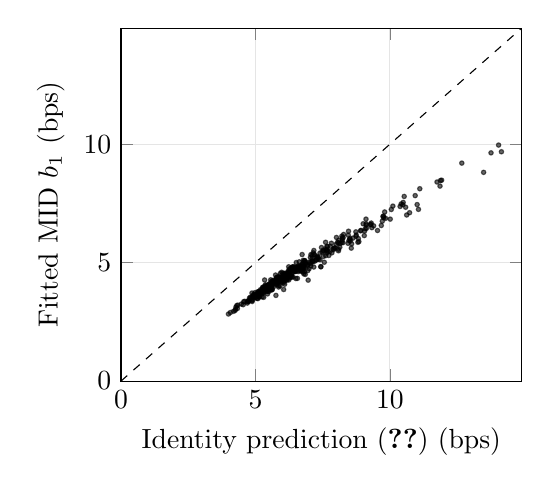
\begin{tikzpicture}
\begin{axis}[width=0.55\textwidth, height=0.5\textwidth, xlabel={Identity prediction \eqref{eq:predict} (bps)},
  ylabel={Fitted MID $b_1$ (bps)}, xmin=0, ymin=0, xmax=14.9, ymax=14.9, grid=major, grid style={gray!20}]
\addplot[only marks, mark=*, mark size=0.8pt, opacity=0.6] coordinates {(5.772,4.151) (5.874,4.189) (5.156,3.665) (4.992,3.641) (6.084,4.421) (5.090,3.482) (6.626,4.667) (6.455,4.752) (5.766,4.278) (4.878,3.361) (7.023,4.996) (5.112,3.767) (5.151,3.655) (8.742,6.113) (5.447,3.680) (6.996,4.746) (5.367,4.063) (4.897,3.588) (5.506,3.875) (9.743,6.946) (8.911,6.344) (5.584,3.877) (6.136,4.381) (8.264,6.056) (8.810,5.861) (10.480,7.449) (5.009,3.531) (5.187,3.736) (6.048,4.148) (5.858,4.182) (6.650,4.833) (8.215,6.123) (5.048,3.626) (6.068,4.506) (5.126,3.698) (5.748,4.478) (5.818,4.391) (5.090,3.773) (5.462,4.043) (7.271,5.230) (5.869,4.370) (5.371,3.878) (5.972,4.173) (6.227,4.448) (8.089,5.502) (6.737,4.756) (5.909,4.362) (4.873,3.427) (7.965,5.621) (5.609,4.165) (6.151,4.259) (6.770,4.672) (5.267,3.923) (4.930,3.594) (3.996,2.832) (5.253,3.804) (5.735,4.205) (7.655,5.414) (7.201,5.335) (6.788,4.797) (6.068,4.487) (6.031,4.200) (5.989,4.220) (5.137,3.546) (6.080,4.230) (6.756,4.851) (5.790,4.309) (13.762,9.637) (6.749,4.930) (5.635,4.105) (8.750,6.166) (8.529,5.914) (4.930,3.639) (6.073,4.532) (6.455,4.632) (5.802,4.110) (5.947,4.249) (4.344,3.208) (5.276,3.846) (6.031,4.384) (5.053,3.491) (7.264,5.106) (5.790,4.192) (5.234,3.734) (6.723,4.768) (6.616,4.789) (7.401,5.122) (7.906,5.553) (4.563,3.350) (6.262,4.619) (5.693,4.196) (7.400,5.406) (6.815,4.796) (10.942,7.832) (5.285,3.719) (6.736,5.344) (6.180,4.534) (5.241,3.815) (5.562,3.930) (6.772,4.894) (5.743,4.196) (6.087,4.090) (5.582,4.197) (9.048,6.144) (6.265,4.419) (11.754,8.406) (6.002,4.228) (8.462,6.328) (7.783,5.691) (5.788,4.083) (5.576,3.841) (7.523,5.262) (5.480,3.904) (6.039,4.313) (6.208,4.618) (6.591,4.625) (5.398,3.980) (6.789,4.754) (6.949,4.666) (5.001,3.536) (4.871,3.718) (6.528,4.794) (11.014,7.453) (9.118,6.643) (5.530,4.111) (6.850,4.950) (5.208,3.727) (5.068,3.686) (6.066,4.398) (5.652,4.071) (6.482,4.648) (6.518,5.005) (5.606,3.916) (14.044,9.966) (8.513,6.022) (8.442,5.818) (5.903,4.262) (5.854,4.326) (12.676,9.205) (8.013,6.065) (5.652,4.191) (5.748,4.223) (5.863,3.971) (5.619,4.094) (6.587,4.744) (6.059,4.344) (8.847,5.888) (5.975,4.595) (10.733,7.110) (10.053,7.246) (6.338,4.775) (9.761,6.969) (5.787,4.231) (6.166,4.429) (5.914,4.018) (5.864,4.344) (7.644,5.536) (6.218,4.543) (8.138,5.653) (7.000,5.022) (7.329,5.189) (10.496,7.544) (8.281,6.193) (5.737,4.237) (4.814,3.470) (6.717,4.856) (5.295,3.857) (4.988,3.736) (5.762,3.618) (6.420,4.721) (8.208,5.851) (9.807,7.141) (5.900,4.296) (6.004,4.408) (5.563,4.057) (6.700,4.642) (5.852,4.030) (5.568,4.276) (10.533,7.797) (6.834,5.082) (9.718,6.752) (6.503,4.331) (5.250,3.551) (6.050,3.867) (6.012,4.548) (6.561,4.337) (5.927,4.232) (9.061,6.336) (7.542,5.490) (5.268,3.959) (6.152,4.374) (4.777,3.499) (6.034,4.486) (6.191,4.539) (4.753,3.375) (4.807,3.541) (6.836,5.082) (5.134,3.703) (6.304,4.733) (6.630,5.035) (7.692,5.476) (6.589,4.784) (6.384,4.816) (6.686,4.797) (7.331,5.235) (6.375,4.587) (6.463,4.782) (6.275,4.417) (6.015,4.301) (4.973,3.547) (9.775,6.899) (6.369,4.818) (7.173,5.514) (6.101,4.558) (5.417,3.833) (4.067,2.895) (5.500,3.874) (4.951,3.670) (10.014,6.839) (5.780,4.333) (5.867,4.396) (8.565,5.614) (7.344,5.145) (7.825,5.820) (4.476,3.251) (7.730,5.305) (8.254,5.844) (4.330,3.067) (6.147,4.397) (5.426,3.892) (5.597,3.992) (7.845,5.416) (5.318,3.800) (6.780,5.099) (6.675,4.661) (5.821,4.179) (4.696,3.293) (5.318,3.982) (5.894,4.225) (7.300,5.254) (8.630,6.039) (8.511,5.983) (6.745,4.817) (6.769,4.602) (8.578,5.797) (5.380,3.773) (5.511,4.061) (6.961,4.261) (6.234,4.657) (4.240,2.982) (8.003,5.771) (5.623,3.861) (5.425,3.845) (4.691,3.354) (5.118,3.675) (6.242,4.269) (9.681,6.570) (8.156,5.810) (5.305,3.908) (7.456,5.640) (6.651,4.742) (4.543,3.224) (5.282,3.859) (5.109,3.598) (7.113,5.074) (10.380,7.374) (8.828,6.017) (9.112,6.840) (4.876,3.546) (13.487,8.814) (6.280,4.374) (6.563,4.821) (5.474,3.946) (4.961,3.616) (7.137,5.073) (7.105,5.314) (8.924,6.364) (14.149,9.684) (5.387,4.035) (5.571,4.076) (5.986,4.273) (7.254,5.122) (7.663,5.511) (6.202,4.506) (5.770,4.205) (5.200,3.820) (7.775,5.471) (7.654,5.685) (5.632,4.115) (6.475,4.760) (6.326,4.416) (7.911,5.594) (11.113,8.122) (7.561,5.018) (7.176,5.343) (7.680,5.678) (7.932,5.620) (5.456,3.787) (6.141,4.434) (10.112,7.390) (5.600,3.949) (5.779,4.278) (10.625,7.013) (8.454,6.158) (5.308,3.538) (5.848,4.259) (9.841,6.871) (5.341,4.269) (4.262,3.030) (5.995,4.279) (6.475,4.719) (4.186,2.946) (5.368,3.852) (6.288,4.479) (8.098,5.945) (5.679,3.993) (6.016,4.332) (4.738,3.395) (6.330,4.477) (6.438,4.832) (5.577,4.049) (9.117,6.591) (7.147,5.414) (5.632,4.237) (5.952,4.253) (6.172,4.273) (5.443,4.015) (8.088,5.569) (6.564,4.792) (7.107,5.175) (8.093,5.837) (7.478,5.452) (11.064,7.251) (6.425,4.702) (6.179,4.450) (9.131,6.453) (6.471,4.643) (8.051,5.856) (5.938,4.288) (6.224,4.484) (5.924,4.545) (6.357,4.519) (4.275,3.124) (6.394,4.797) (5.556,3.880) (7.123,5.044) (5.472,3.830) (5.296,3.955) (9.396,6.556) (5.489,4.059) (6.661,4.870) (5.119,3.770) (7.435,4.824) (5.098,3.673) (5.481,4.070) (5.505,3.918) (8.736,6.301) (6.858,4.912) (5.150,3.559) (7.056,4.958) (7.522,5.531) (8.477,5.935) (5.496,3.782) (6.266,4.350) (6.394,4.391) (6.380,4.680) (6.854,4.505) (5.685,4.259) (7.609,5.861) (8.228,6.048) (7.612,5.296) (5.868,4.234) (5.876,4.378) (5.484,3.953) (5.185,3.856) (9.306,6.673) (9.540,6.359) (6.801,5.054) (6.301,4.637) (5.105,3.568) (6.857,5.001) (11.926,8.483) (5.936,4.342) (11.883,8.468) (6.761,4.946) (5.902,4.295) (6.753,4.812) (6.236,4.825) (10.587,7.340) (10.421,7.482) (6.266,4.737) (6.937,4.920) (7.059,4.860) (5.297,3.736) (5.170,3.633) (5.415,3.987) (8.230,5.964) (6.931,4.869) (4.996,3.576) (6.828,4.621) (9.084,6.433) (6.351,4.396) (4.935,3.549) (5.131,3.734) (5.929,4.264) (9.007,6.642) (7.430,4.835) (4.732,3.359) (6.167,4.335) (6.397,4.775) (7.620,5.571) (9.289,6.612) (5.210,3.699) (6.802,4.525) (7.191,5.053) (4.305,3.187) (7.171,4.816) (4.598,3.369) (5.787,4.378) (9.277,6.605) (6.596,4.844) (7.042,5.223) (9.330,6.477) (5.395,3.861) (6.501,4.628) (5.862,4.398) (11.865,8.234) (4.875,3.401) (5.955,4.256) (7.064,5.340) (5.616,3.866)};
\addplot[dashed, domain=0:14.9] {x};
\end{axis}
\end{tikzpicture}
\caption{Each point is a stock. The dashed line is the 45-degree line. The fitted $b_1$ lines up with a
number that is computed without any regression.}
\label{fig:scatter}
\end{figure}

\paragraph{Test 1: the identity explains the pattern across stocks.} The fitted $b_1$ and the prediction
correlate $0.989$ (Figure~\ref{fig:scatter}). The fitted value is below the prediction on average
because the regression also contains the lags of $r$ and $x$, which absorb part of the same variation.
What matters is that knowing where closes sit within their ranges in a stock almost fully tells us that
stock's $b_1$.

\paragraph{Test 2: the coefficient does not survive the control.} Adding one regressor removes
$97\%$ of $b_1$ and the share of significant stocks falls from $100\%$ to $38\%$.
$R^2$ rises from $0.348$ to $0.594$: most of what the MID regression explained was the known
term. $b_0$ does not move, which shows that the control removes the identity and nothing else.

\paragraph{Test 3: no identity, no coefficient.} With CLOSE, $b_1 =$ $0.025$ bps.

\subsection{The same mechanism explains $a_1$ and the impulse response}

The MID $a_1$ is $0.18$ while the CLOSE $a_1$ is $-0.013$. Averaging prices over a bar makes their
changes positively autocorrelated \citep{working1960}; closing prints bounce between bid and ask and
make changes negatively autocorrelated \citep{roll1984}. Neither is the true price.

\begin{figure}[htbp]
\centering
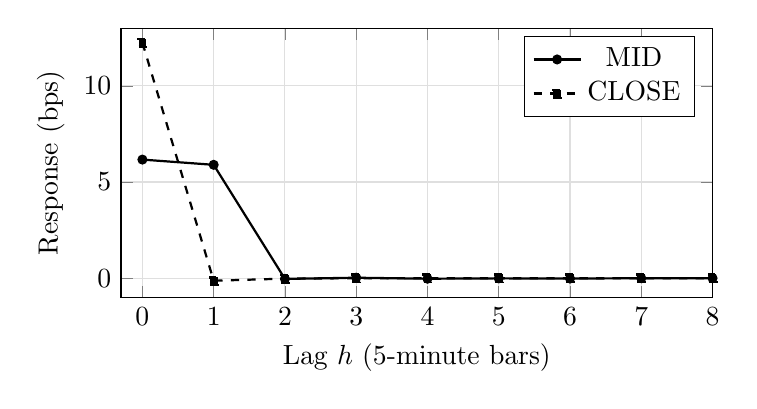
\begin{tikzpicture}
\begin{axis}[width=0.75\textwidth,height=5cm, xlabel={Lag $h$ (5-minute bars)}, ylabel={Response (bps)},
  legend pos=north east, grid=major, grid style={gray!25}, xmin=-0.3, xmax=8, ymin=-1, ymax=13]
\addplot[thick,mark=*,mark size=1.4pt] coordinates {(0,6.1673) (1,5.8956) (2,-0.0381) (3,0.0229) (4,-0.0282) (5,-0.0105) (6,-0.0197) (7,-0.0034) (8,0.0000)}; \addlegendentry{MID}
\addplot[thick,dashed,mark=square*,mark size=1.4pt] coordinates {(0,12.2493) (1,-0.1342) (2,-0.0238) (3,-0.0063) (4,-0.0058) (5,-0.0087) (6,0.0008) (7,0.0001) (8,-0.0000)}; \addlegendentry{CLOSE}
\end{axis}
\end{tikzpicture}
\caption{Impulse response \eqref{eq:irf} from the average coefficients. Cumulative responses:
$11.99$ bps (MID) and $12.07$ bps (CLOSE).}
\label{fig:irf}
\end{figure}

Figure~\ref{fig:irf} gives the decisive check. If MID kept information that CLOSE loses, its total response
would be larger. The totals are $11.99$ and $12.07$ bps, the same. MID only spreads the same
response over two bars instead of one, which is exactly what a price that lags the close by part of a
bar should do.

\subsection{What survives}

After the control, $b_1$ is $0.128$ bps and significant in $38\%$ of stocks, almost always positive. The remaining coefficient is a genuine but small carry-over of impact into the next bar, $37$ times smaller
than the raw coefficient, and $3.7$ times smaller than the smallest cost of a single trade
(half of one \$0.01 tick at the median stock price).

%=====================================================================
\section{The two-step forecast is not identified}
\label{sec:twostep}

To forecast $r_{t+1}$ with \eqref{eq:price} one needs $x_{t+1}$, which is unknown at time $t$. A popular
construction first forecasts it and then uses the forecast:
\begin{align*}
\text{Step A:}\quad & \hat x_{t+1} = \Phi_t\,\hat\beta_x, \qquad \Phi_t=[1,\ r_t,\dots,r_{t-L+1},\ x_t,\dots,x_{t-L+1}],\\
\text{Step B:}\quad & \hat r_{t+1} = \Phi_t\,\hat\beta + \delta\,\hat x_{t+1},
\end{align*}
with $\delta$ read as ``how much expected order flow moves expected returns beyond the lags''.

\begin{proposition}[Degeneracy]
\label{prop:twostep}
If Step A uses the same regressors as Step B, then $\hat x = \Phi\hat\beta_x$ lies in the column space of
$\Phi$. Hence (i) $[\Phi,\hat x]$ has rank equal to the number of columns of $\Phi$, one less than its own
number of columns; (ii) the fitted values of Step B equal those of the plain regression of $r$ on $\Phi$;
(iii) $\delta$ is not identified: for any $s$, replacing $(\hat\beta,\delta)$ by
$(\hat\beta - s\hat\beta_x,\ \delta+s)$ leaves every fitted value unchanged.
\end{proposition}
\begin{proof}
(i) $\hat x$ is a linear combination of the columns of $\Phi$, so adding it adds no new direction.
(ii) Least-squares fitted values are the projection of $r$ on the column space, which is unchanged by (i).
(iii) $\Phi(\hat\beta-s\hat\beta_x)+(\delta+s)\Phi\hat\beta_x = \Phi\hat\beta+\delta\,\Phi\hat\beta_x$.
\end{proof}

The same holds for the ARX used for forecasting: substituting the flow equation into the price equation
gives a forecast linear in $\Phi_t$ with coefficients $a_k+b_0c_k$ on returns and $b_k+b_0d_k$ on flow, so
the one-step regression of $r_{t+1}$ on $\Phi_t$ already is the VAR forecast.

\paragraph{Empirical check.} We ran both versions in a rolling walk-forward (1-year window, monthly
refits) on every stock: 17{,}240 refits. In every refit the augmented matrix has rank 11
with 12 columns, and the two forecasts differ by at most $1.9\times10^{-11}$ bps, i.e.\ they are the
same numbers.

\paragraph{What software reports.} Statistical software does not refuse a singular design; it returns
the minimum-norm solution of the pseudo-inverse and a standard error computed from it. In our runs this
``$\delta$'' is positive in $91.5\%$ of refits and has $|t|>2$ in $44\%$. The reported $\delta$ and its $t$-statistics describe the pseudo-inverse, not the data. A reader who sees them cannot tell that $\delta$ does not exist.

\paragraph{A version that is identified.} If Step A uses information that Step B does not have, here five
lags of log volume and of the bar's range, $\hat x$ leaves the column space and $\delta$ can be estimated. The coefficient $\delta$ is then clearly positive (mean $21.9$, positive in $98\%$ of refits, $|t|>2$ in $83\%$):
expected order flow does move expected returns. The extra term still does not help forecasting, because $\delta$
multiplies $\hat x$, whose standard deviation is only about $\sqrt{R^2}=$ $0.020$ of that of $x$. A
coefficient can be real and precisely estimated and still move the forecast by almost nothing.

%=====================================================================
\section{A test for bar-level regressions}
\label{sec:checklist}

The two identities are special cases of a general rule. Any statistic of a bar is a function of the same
five numbers $(O,H,L,C,V)$, so two statistics of the same bar are mechanically related. If the price is
an interior statistic of the bar (range midpoint, $(H+L+C)/3$, VWAP), the decomposition \eqref{eq:decomp}
moves part of bar $t$ into the return of bar $t+1$, and the relation appears at lag one. If the price is
a rolling average over $k$ bars, it appears up to lag $k$ and looks like slowly decaying impact. The
following steps catch this before a result is interpreted.

\begin{enumerate}
\item \textbf{Write the identity.} Decompose the target through bar endpoints, as in \eqref{eq:decomp},
and find any term that is known at time $t$.
\item \textbf{Predict the coefficient without the regression}, as in Proposition~\ref{prop:b0} or
\eqref{eq:predict}, and correlate the prediction with the fitted coefficient across assets.
\item \textbf{Control for the known term} and report the coefficient before and after.
\item \textbf{Check the rank} of any design that contains a fitted value from an earlier regression.
\item \textbf{Score forecasts on a return that a trade can earn}, never only on the model's own target.
\end{enumerate}

Each step is cheap enough to run on every new feature. Standard diagnostics do not help: an identity has large $t$-statistics, replicates across
assets, survives robust standard errors and out-of-sample tests, and raises $R^2$.

%=====================================================================
\section{Limitations}
\label{sec:limits}

The results rest on bar data, one market and one period; each limit below states what that excludes.


\paragraph{No trade data.} The paper shows what the bar version measures; it cannot show what the
trade-level version would find on the same stocks. The natural next step is to sign trades with
\citet{lee1991} and run \eqref{eq:price}--\eqref{eq:flow} on trade time.

\paragraph{One frequency and one market.} Everything is 5-minute US large caps. The identities do not
depend on the frequency, but the size of the residual effect in Section~\ref{sec:b1} does.

\paragraph{Survivorship.} The sample contains stocks with data for the whole period. Survivorship is unlikely to affect the identities, which hold bar by bar, but the averages describe surviving large caps.

%=====================================================================
\section{Conclusion}

On 5-minute bars the Hasbrouck VAR produces results that look like strong evidence of information in
trades and are mostly arithmetic. With close prices the contemporaneous coefficient is a function of the
size of 5-minute moves; with range-midpoint prices the lagged coefficient is a known term moved by one
bar; order flow cannot be forecast; and the two-step forecast built on the VAR is not identified.
Information in trades is real, but these bars cannot show it. Work with bar data should decompose the
target, predict the suspect coefficient without the regression, and control for the known term before
reading any coefficient as economics.

\begin{thebibliography}{99}
\bibitem[Glosten and Milgrom(1985)]{glosten1985} Glosten, L.~R. and Milgrom, P.~R. (1985). Bid, ask and transaction prices in a specialist market with heterogeneously informed traders. \emph{Journal of Financial Economics}, 14(1), 71--100.
\bibitem[Hasbrouck(1991)]{hasbrouck1991} Hasbrouck, J. (1991). Measuring the information content of stock trades. \emph{Journal of Finance}, 46(1), 179--207.
\bibitem[Hasbrouck(2007)]{hasbrouck2007} Hasbrouck, J. (2007). \emph{Empirical Market Microstructure}. Oxford University Press.
\bibitem[Kyle(1985)]{kyle1985} Kyle, A.~S. (1985). Continuous auctions and insider trading. \emph{Econometrica}, 53(6), 1315--1335.
\bibitem[Lee and Ready(1991)]{lee1991} Lee, C.~M.~C. and Ready, M.~J. (1991). Inferring trade direction from intraday data. \emph{Journal of Finance}, 46(2), 733--746.
\bibitem[Newey and West(1987)]{newey1987} Newey, W.~K. and West, K.~D. (1987). A simple, positive semi-definite, heteroskedasticity and autocorrelation consistent covariance matrix. \emph{Econometrica}, 55(3), 703--708.
\bibitem[Roll(1984)]{roll1984} Roll, R. (1984). A simple implicit measure of the effective bid-ask spread in an efficient market. \emph{Journal of Finance}, 39(4), 1127--1139.
\bibitem[Working(1960)]{working1960} Working, H. (1960). Note on the correlation of first differences of averages in a random chain. \emph{Econometrica}, 28(4), 916--918.
\end{thebibliography}

\end{document}
